
\section{\ref{PS:Q:Feasibility}}
\subsection{Experimenit}

The \ref{PS:Q:Feasibility} question asks if it is possible to re-implement the current system at Siemens Wind Power as a decentralized system. The following experiment aims to investigate if the proposed decentralized system can perform the operations that the current centralized system at Siemens Wind Power is able to perform. More specifically the experiments aims to investigate if the proposed decentralized system is able to regulate the power production of each turbine in order to maintain the global power production goal.
The experiment has the following procedure:
\begin{enumerate}
	\item Start the system with 100 turbines.
	\item Start the graphical interface described in \cref{sec:graphicalInterface}.
	\item Observe that the global setpoint and the global production line on the graphical interface match.
\end{enumerate}








\subsection{Result}
\label{sec:exp:feasibility}
\begin{figure} [!h]
	\centering
	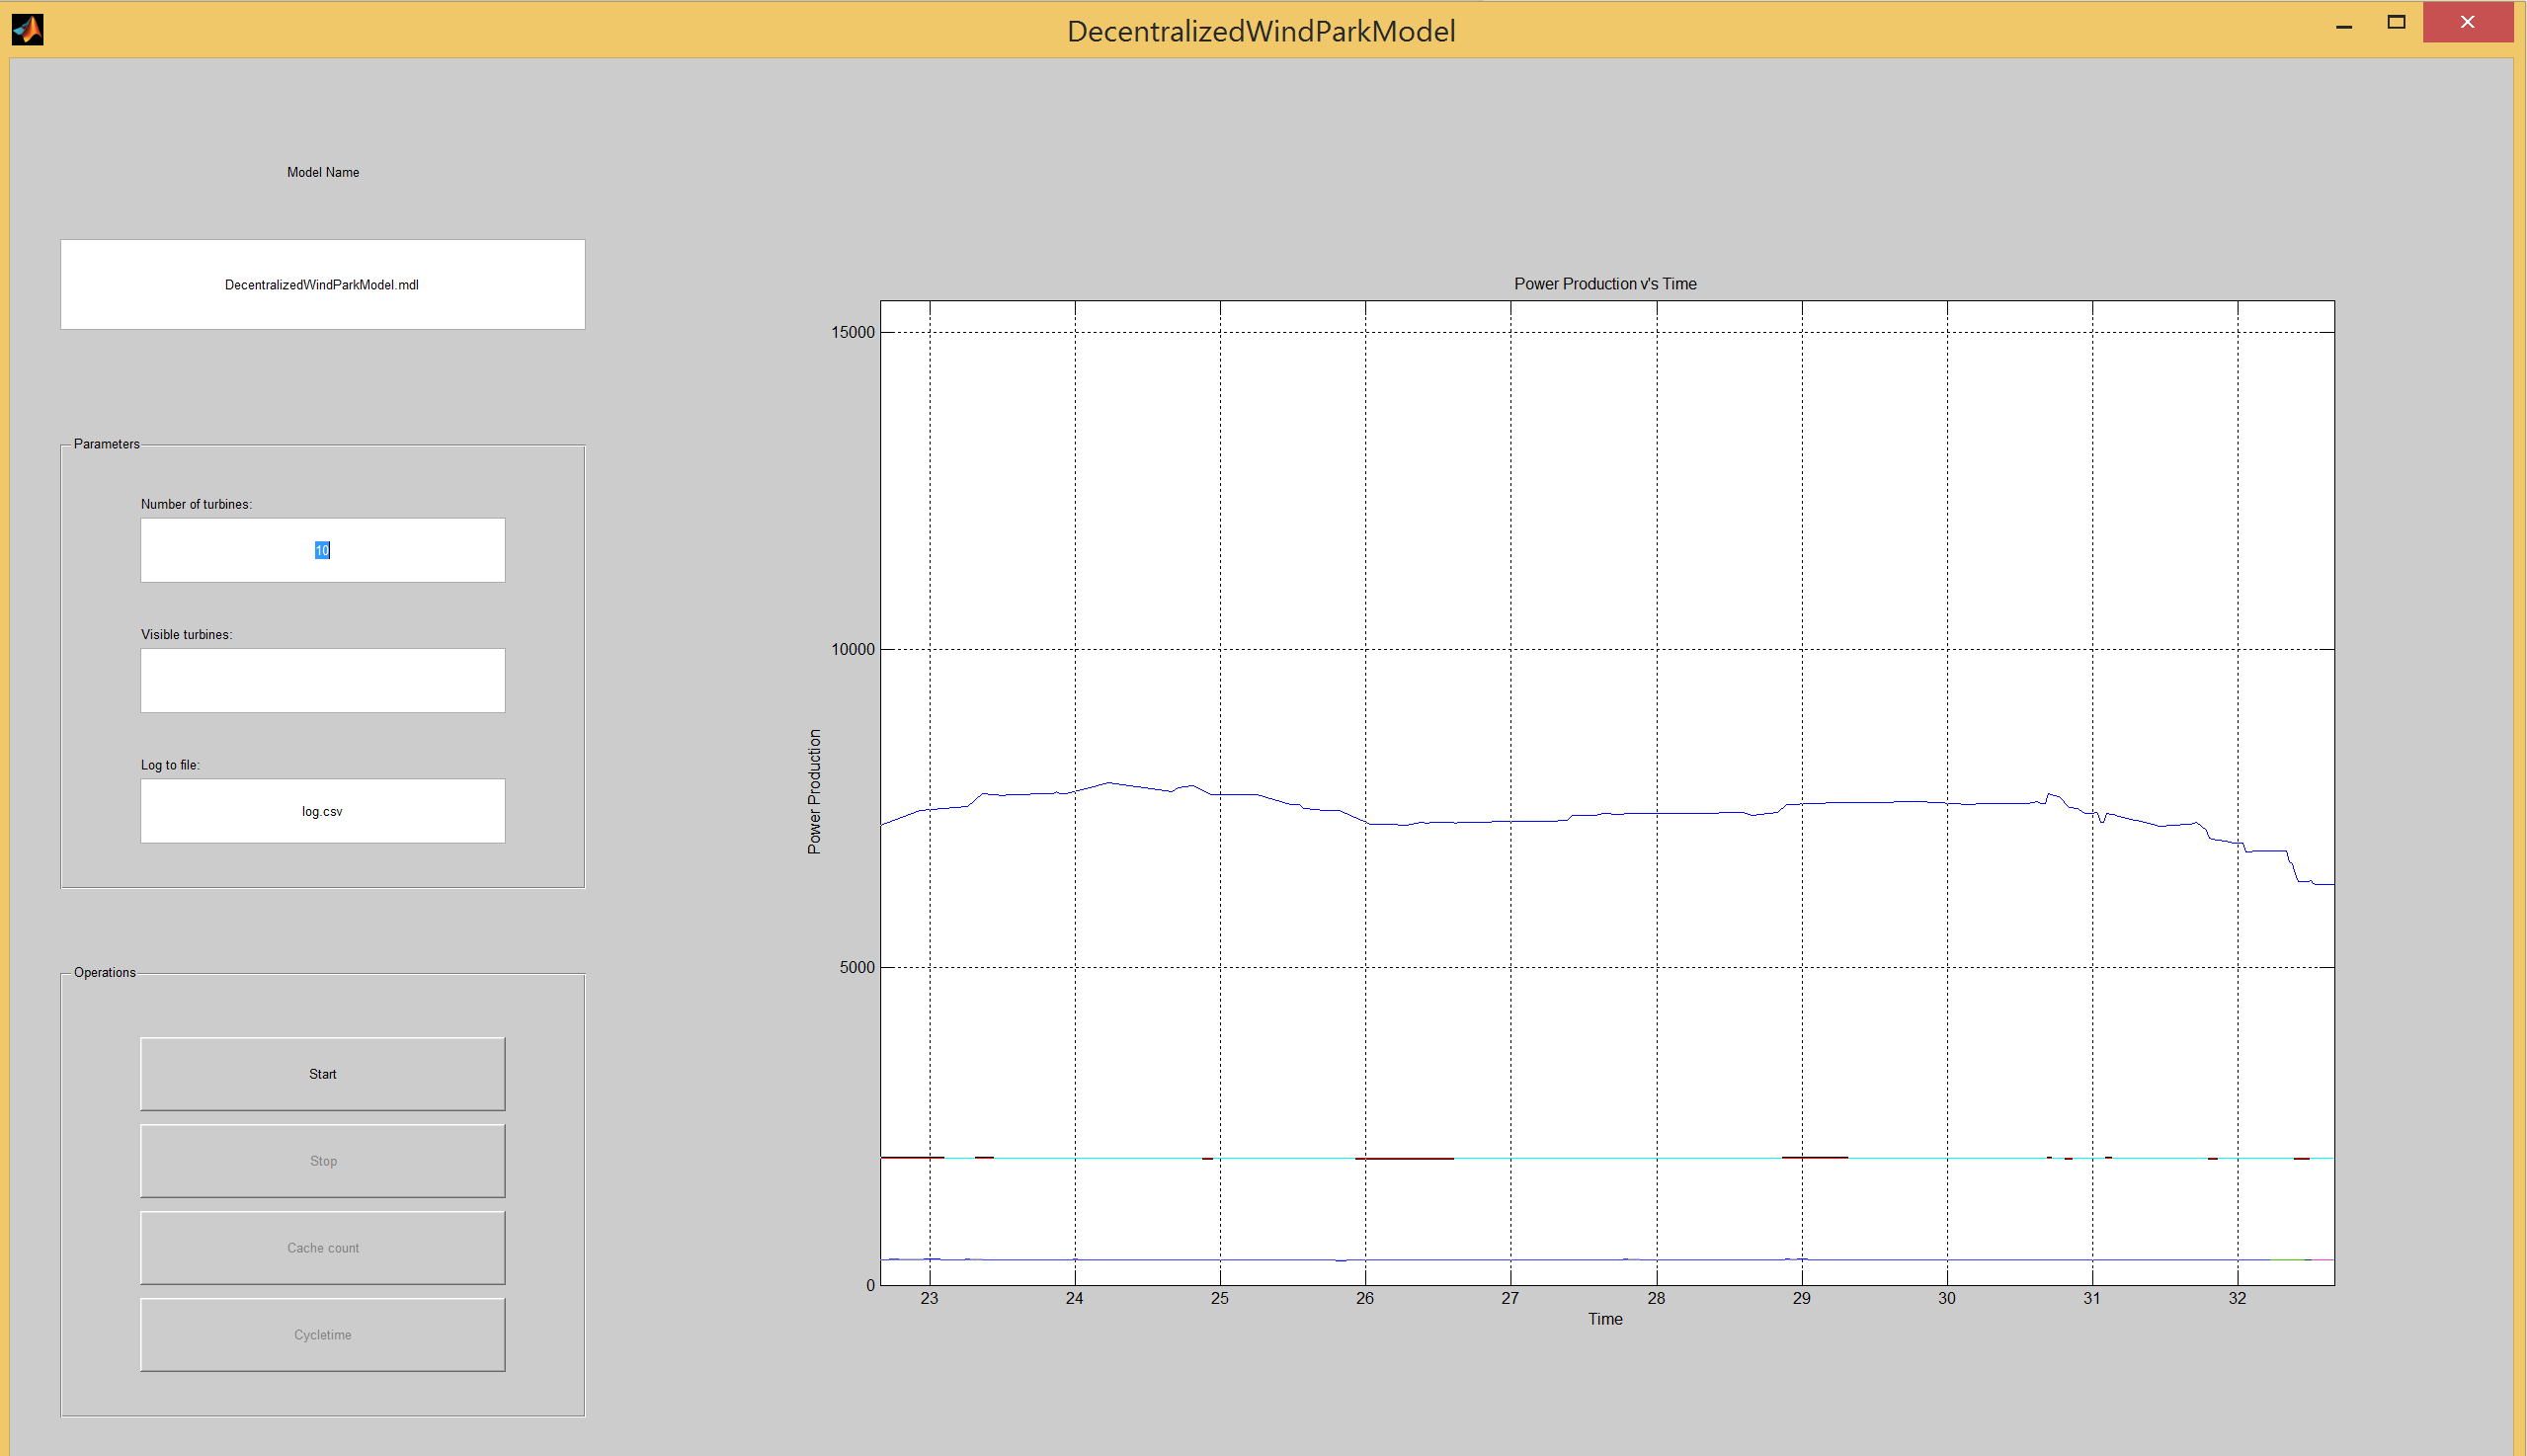
\includegraphics[width=\resultsFigureWidthScale\textwidth]{gui.png} 
	\captionsetup{format=plain,font=footnotesize,labelfont={bf,defaultCapFont},labelsep=quad,singlelinecheck=no}
	\caption[Graphical interface running 5 turbines]{
		\label{fig:graphicalInterface} 
		\footnotesize{%
			Graphical interface running 5 turbines.
		}
	}
\end{figure}
Presented in \cref{fig:graphicalInterface} is shown a screenshot of the graphical interface while the decentralized solution is running 5 turbines.
The global setpoint for power production is at 2000, illustrated by the red line and global power production is illustrated by the black line.
The blue line illustrates the maximum available power production for the wind farm while the lines in the bottom around 400 is the power production of each individual turbine.

\subsection{Discussion}
